\newpage
\section{Tieftöner-Verstärker}\label{kap:5.3}
\subsection{Allgemeines}\label{kap:5.3.1}
Nach dem Filtern des Signals soll dieses vor dem Abstrahlen am Lautsprecher verstärkt werden. Es wurde eine analoge Verstärker-Schaltung verwendet, da diese einfacher und mit weniger Problemen realisiert werden hat können. Mit Hilfe bereits bekannter, bewährter Schaltungen konnte ein Layout für diese Schaltung designet werden. Ein wichtiger Baustein in dieser Schaltung ist der Verstärker \enquote{TDA2030}, wie in Kapitel \ref{kap:5.3.3} beschrieben.  Des weiteren wurden zwei Leistungstransistoren verbaut die höhere Ströme schalten können, falls der maximale Schaltstrom des TDA2030 erreicht wird.

\subsection{Zielsetzung}\label{kap:5.3.2}
Das Eingangssignal soll Verstärkt werden um am Ausgang der Schaltung höhere Spannungs-Amplituden und höheren Ströme aufzuweisen. Es soll nach diesem Schritt möglich sein den Tieftöner in einer der zwei Satellitenboxen mit ausreichend Signal zu versorgen, um einen Schalldruck von zumindest Zimmerlautstärke zu erhalten. 

\subsection{TDA2030}\label{kap:5.3.3}
Der TDA2030 ist ein für den Audio-Frequenzbereich optimierter OPV. Dieser kann symmetrisch sowie auch asymmetrisch versorgt werden. Eine typische Beschaltung ist im Datenblatt auch vorgegeben, welche auch verwendet wurde. Der TDA2030 besitzt ein Pentawatt-Gehäuse, welches deshalb auch eine Kühlfläche besitzt. Diese Kühlfläche hat das selbe Potential wie der mittlere Anschlusspin (Abb. \ref{5.3.3.1}).\\
Es wird auch für geringfügigen Betrieb ein Kühlkörper empfohlen!
\begin{figure} [ht]
	\centering
	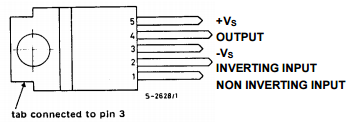
\includegraphics[width=1\textwidth]{img/Print5/TDA2030Pinning.PNG}
	\caption{TDA2030-Pinning}
	\label {fig:abb5.3.3.1}
\end{figure}
\subsubsection{Absolute Maximalwerte}
Diese Werte wurden zu aller erst mit den Bedingungen an der Schaltung verglichen, da sie ein sehr genaue, kurze Übersicht über den Baustein liefern.
\begin{figure} [ht]
	\centering
	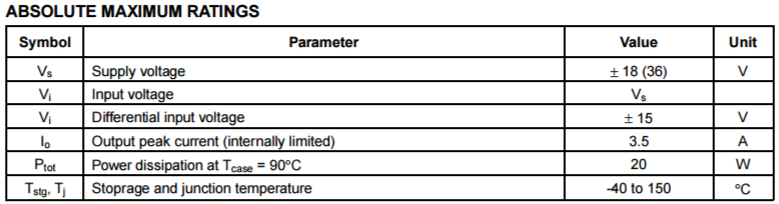
\includegraphics[width=1\textwidth]{img/Print5/TDA2030MaximumRatings.PNG}
	\caption{TDA2030-Pinning}
	\label {fig:abb5.3.3.2}
\end{figure}

\begin{comment}
\begin{figure} [ht]
	\centering	
	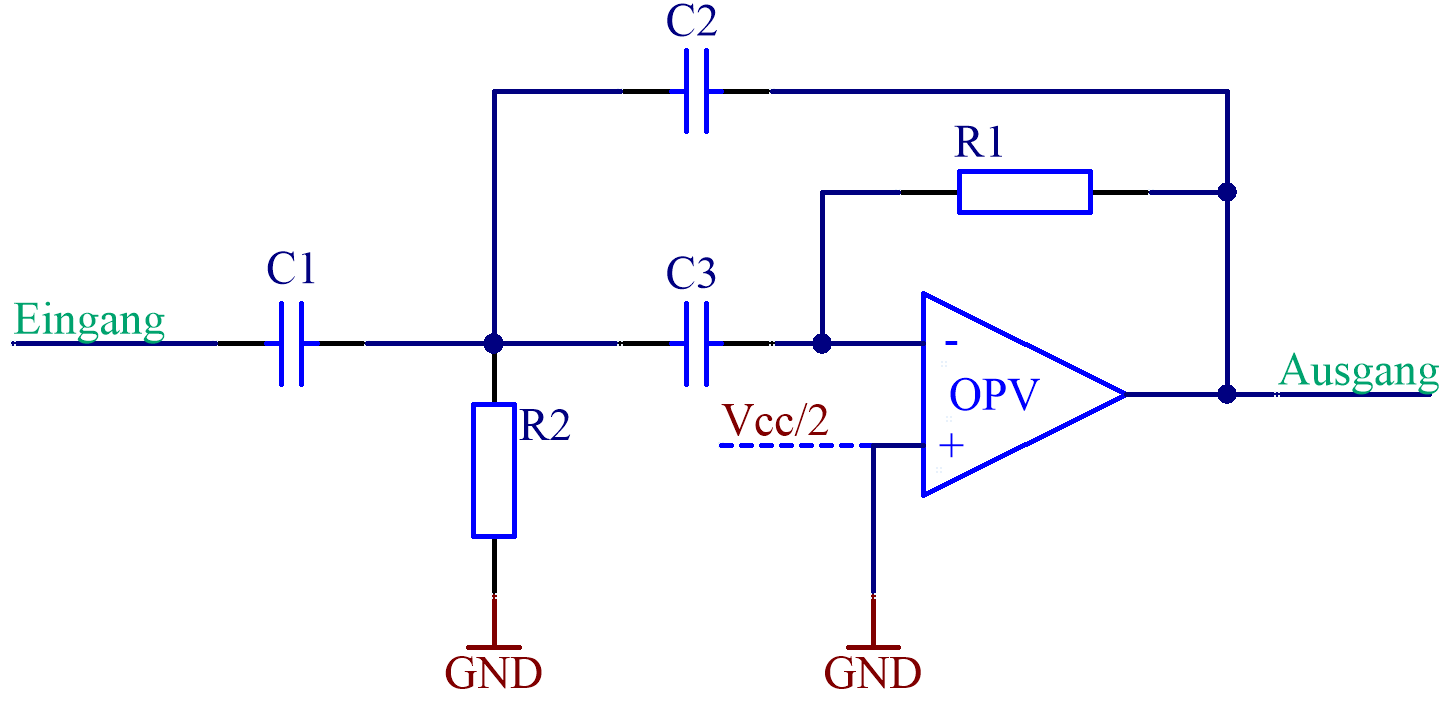
\includegraphics[width=1\textwidth]{img/Print4/HPFilter-Butterworth2Ordnung.PNG}
	\caption{Butterworth-Hochpass-Filter 2. Ordnung}
	\label {fig:abb5.2.3.2}
\end{figure}

\subsection{Schaltung}\label{kap:5.2.4}

Das Eingangssignal (Links, Rechts, Masse) wird an einer dreipoligen Stifleiste angeschlosssen (Abb. \ref{fig:abb5.2.4.1}). Zuerst gelangt Signal-Links und -Rechts an jeweils ein Potentiometer um den Pegel anpassen zu können, es bietet also eine Regelmöglichkeit. Es folgen die Filter. Hochpass für Links/Rechts und Tiefpass für Links/Rechts. Ein \enquote{Butterworth-Tiefpass-Filter 2. Ordnung} wurde bereits in dem Kapitel \ref{kap:5.1.4} erklärt. Das \enquote{Butterworth-Hochpass-Filter und -Bandpass-Filter 2. Ordnung} weist keine groben Unterschiede auf, der Unterschied liegt lediglich in der Bauteilaufteilung.\\
Nach den Filtern gelangen die getrennten Signale zu deren Ausgangspunkt. Es ist für jede Signalleitung eine zweipolige Stiftleist vorgesehen (Signal + Masse), da der darauffolgende Verstärker einen selbigen Eingang besitzt. Die Stiftleisten sind jedoch gruppiert nach Bandpass- und Hochpass-Ausgang.\\
\begin{figure} [ht]
	\centering	
	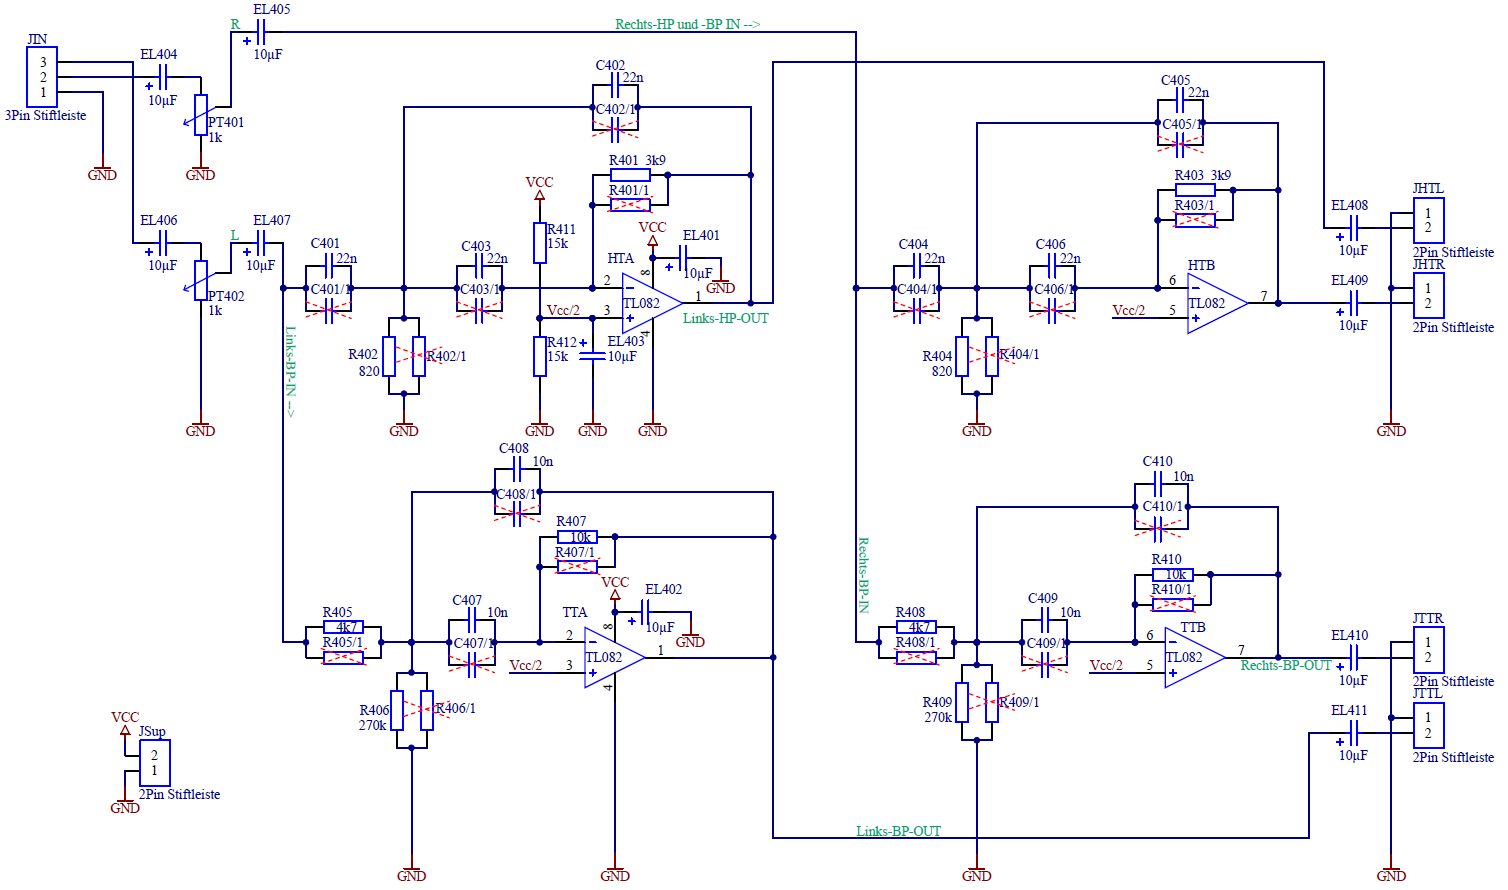
\includegraphics[width=1\textwidth]{img/Print4/4_TTuHTWeiche-Schematic.PNG}
	\caption{Butterworth-Bandpass-Filter 2. Ordnung}
	\label {fig:abb5.2.4.1}
\end{figure}\\
Eines der Bandpass-Filter. Gut sichtbar die doppelte, parallele Ausführung von Widerständen und Kondensatoren um krumme Werte auch erhalten zu können. Bedingt durch Parallel-Schaltung von Widerständen und Kondensatoren.\\ 
Der Eingang wurde gespiegelt um ein schöneres Bild zu erlangen. Die Spiegelung ist für das PCB-Layout nicht relevant!\\
Bedingt durch die Versorgungsspannung ist auch der Spannungsteiler für $\frac{Vcc}{2}$ am Plus-Eingang des OPVs implementiert.
\begin{figure} [ht]
	\centering	
	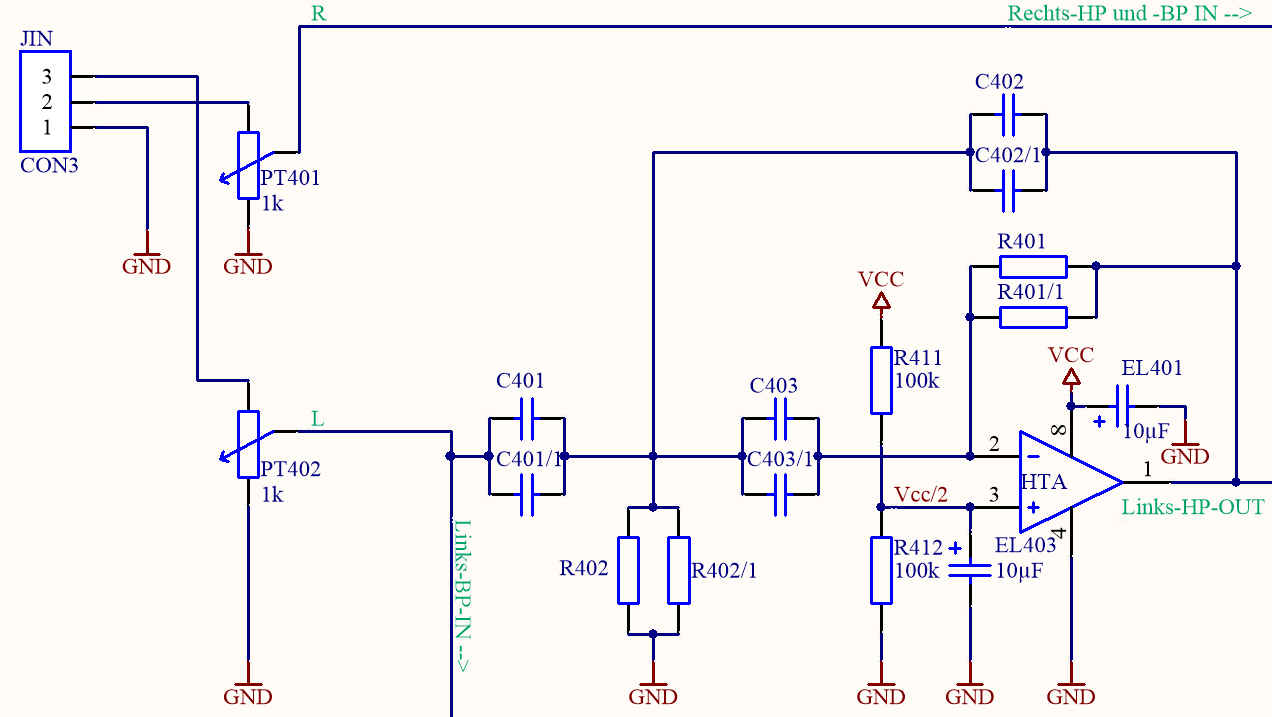
\includegraphics[width=1\textwidth]{img/Print4/4_TTuHTWeiche-LinksHP-Schematic.PNG}
	\caption{Butterworth-Bandpass-Filter 2. Ordnung - aus Abb.\ref{fig:abb5.2.4.1}}
	\label {fig:abb5.2.4.2}
\end{figure}\\
Am B-Teil des OPVs (erkennbar an der Beschriftung: TT\enquote{B}) ist keine Versorgung einzuzeichnen, da er mit dem A-Teil einen achtpinnigen IC mit zwei integrierten OPVs ergibt. Die zwei Teile sind über das IC-Gehäuse mit der gleichen Versorgungsspannung verbunden, deshalb ist das einmalige Kennzeichnen ausreichend.\\
\begin{figure} [ht]
	\centering	
	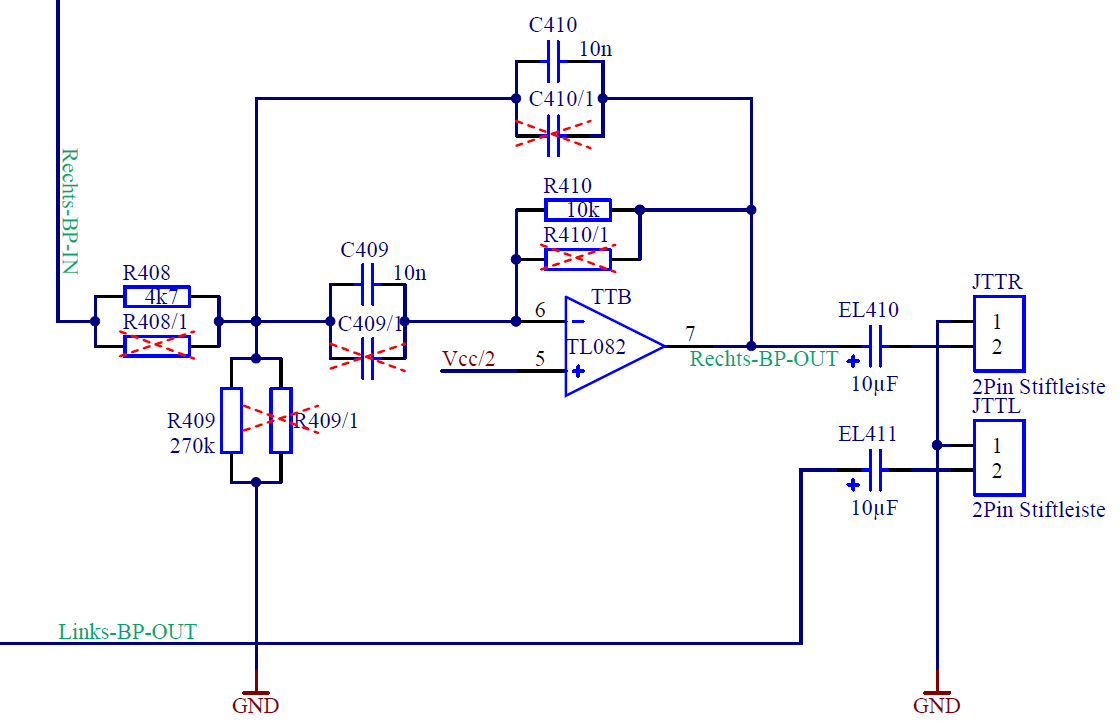
\includegraphics[width=1\textwidth]{img/Print4/4_TTuHTWeiche-RechtsBP-Schematic.PNG}
	\caption{Butterworth-Bandpass-Filter 2. Ordnung - aus Abb.\ref{fig:abb5.2.4.1}}
	\label {fig:abb5.2.4.3}
\end{figure}

\subsection{PCB}\label{kap:5.2.5}
Es wurden die grundlegenden Regeln zur Leiterplattenentflechtung angewandt (\ref{}). Bei dem Design (Abb. \ref{fig:abb5.2.5.1}) wurde auf hohe Variierbarkeit geachtet um auch zB. Kondensatoren mit unterschiedlichen Footprint verwenden zu können.\\
Es wurden wieder nahe an den IC's ELKOs in der Spannungsversorgungsleitung verbaut, um Störungen zu verhindern.

\begin{figure} [ht]
	\centering	
	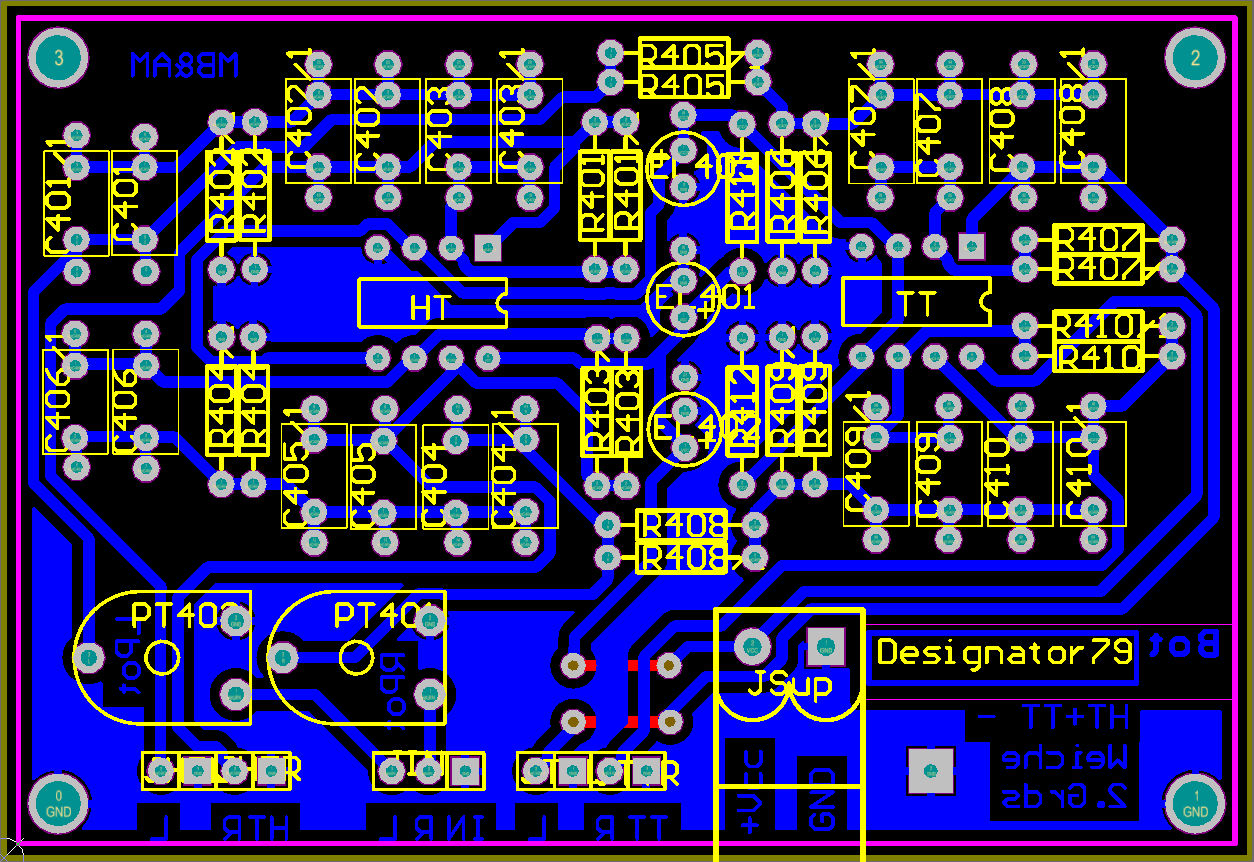
\includegraphics[width=1\textwidth]{img/Print4/4_TTuHTWeiche-PCB.PNG}
	\caption{Tieftöner- und Hochtönerweichen - PCB}
	\label {fig:abb5.2.5.1}
\end{figure}


\begin{comment}
%% Altium und Einstellungserklärung + Wichtige Layout-Faktoren
%Beim designen des Leiterplattenlayouts wurden die allgemeinen Altium-Einstellungen vorgenommen und auf die zu berücksichtigenden Layoutpunkte geachtet.
Beim \enquote{Layouten} der Schaltung mussten einige wichtige Faktoren berücksichtigt werden.\\
Wie da wären:\\
\begin{itemize}
	\item EMV-Technische-Faktoren, wie kurze Leiterbahnen
	\item Ausnützen der Printfläche
	\item Mehrfach-Footprints ermöglichen für verschiedene Bauteile
	\item Mechanische Aufhängebohrungen vorsehen
	\item Massefläche bei Möglichkeit vorsehen
\end{itemize}
Leiterplattenspezifische Einstellungen wurden aus den Kriterien der schuleigenen Leiterplattenfertigung übernommen. Zu diesen Einstellungen zählen:\\
\begin{itemize}
	\item Leiterbahnbreite
	\item Leiterbahnabstände untereinander
	\item Restring bei Bohrungen
	\item 
\end{itemize}
\end{comment}






